\DiaryEntry{Inside Interesting Integrals, 6 (Section 2.4)}{2018-03-21}{Integrals}

This is a continuation of Journal entry \ref{2016-02-17:entry}. Final result there is

\be
\label{2018-03-21:eq1}
\int_0^{\pi/2} \ln(a \sin x) dx = \frac{\pi}{2} \ln \frac{a}{2}
\ee

We will use this result to calculate the integral

\bee
I = \int_{0}^{\pi/2} \ln \left\{\frac{\sin(x)}{x} \right\} dx
\eee

We can rewrite the integral as

\bee
I = \int_{0}^{\pi/2} \ln \left( \sin(x) \right) dx - \int_{0}^{\pi/2} \ln \left( x \right) dx
\eee

Setting $a=1$ in \eqref{2018-03-21:eq1}, we get $\int_0^{\pi/2} \ln(\sin x) dx = \frac{\pi}{2} \ln \frac{1}{2}$ for the first integral. Furthermore, we have $\int \ln(x) dx = x \ln(x)-x$, and we arrive at

\bee
I = \frac{\pi}{2} - \left. \left( x \ln(x) - x \right) \right|_{0}^{\pi/2} = \frac{\pi}{2} - \left[ \frac{\pi}{2} \ln\frac{\pi}{2} - \frac{\pi}{2}  - 0 \right] = \frac{\pi}{2} - \frac{\pi}{2} \log \pi
\eee

So we have

\bee
\boxed{
I = \int_{0}^{\pi/2} \ln \left\{\frac{\sin(x)}{x} \right\} dx = \frac{\pi}{2} (1 - \log \pi) \approx -0.277
} \qed
\eee

The integrand is shown in the following Figure:

\begin{figure}[H]
	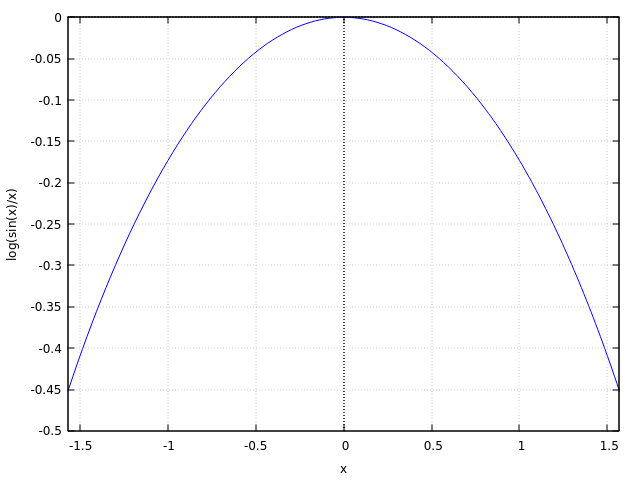
\includegraphics[scale=0.7]{images/interesting_integrals_06_1.png}
\end{figure}

We next observe

\bee
1 + \tan^2 \phi= \frac{1}{\cos^2 \phi}
\eee

and taking the log on both sides yields

\bee
\ln(1 + \tan^2 \phi) = \ln(\frac{1}{\cos^2 \phi})
\eee

and we further obtain

\bee
\ln(\cos \phi) = -\frac{1}{2} \ln(1 + \tan^2 \phi)
\eee

From the Journal entry \ref{2016-02-17:entry} we also have 

\bee
\int_0^{\pi/2} \ln(a \sin x) dx = \int_0^{\pi/2} \ln(a \cos x) dx = \frac{\pi}{2} \ln \frac{a}{2}
\eee

Inserting above relation into the integral, we obtain

\bee
\int_0^{\pi/2} \ln(\cos x) dx = \int_0^{\pi/2} -\frac{1}{2} \ln(1 + \tan^2 x) dx = \frac{\pi}{2} \ln \frac{1}{2} = - \frac{\pi}{2} \ln 2
\eee

which can be simplified to

\bee
\int_0^{\pi/2} \ln(1 + \tan^2 x) dx = \pi \ln 2
\eee

Next, we perform the substitution $u = \tan x$ with $\frac{du}{dx} = \frac{1}{\cos^2 x}$ and therefore

\bee
dx = \cos^2 x du = \frac{1}{1 + \tan^2 x} du = \frac{du}{1 + u^2}dx
\eee

Here we have used "standard trick" to use the original substitution in expressing $dx$. Using this, we obtain

\be
\label{2018-03-21:eq2}
\boxed{
\int_0^\infty \frac{ \ln(1 + u^2)}{1+u^2} du = \pi \ln 2 \approx 2.178
}
\ee

where we have transformed the limits as follows $x=0 \rightarrow u = \tan 0 = 0$ and $x=\pi/2 \rightarrow u = \tan \pi/2 = \infty$. The following Figure shows a plot of the integrand.

\begin{figure}[H]
	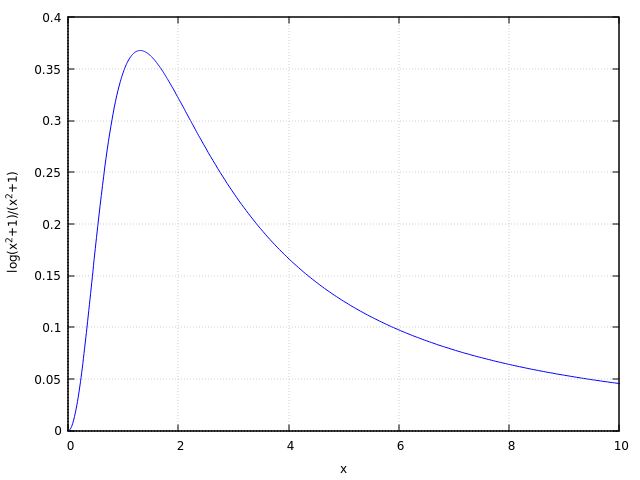
\includegraphics[scale=0.7]{images/interesting_integrals_06_2.png}
\end{figure}


We can plot and calculate the integral in Maxima as follows

\begin{verbatim}

(%i1)	plot2d(log(1+x^2)/(1+x^2), [x,0,10]);
(%o1)	["/tmp/maxout6311.gnuplot_pipes"]
(%i2)	romberg(log(1+x^2)/(1+x^2), x, 0, 200);
(%o2)	2.11460420524655
(%i3)	quad_qag(log(1+x^2)/(1+x^2), x, 0, 1e5, 1);
(%o3)	[2.17733583179431,8.391913884226576*10^-12,525,0]
(%i4)	float(%pi*log(2)), numer;
(%o4)	2.177586090303602

\end{verbatim}

\qed

We can use this result to solve some other integral. We first split the integral into $\int_0^1 + \int_1^\infty$ and substitute $u = 1/x$ in the second one. We have $du/dx=-1/x^2 \rightarrow dx = -x^2 du = -1/u^2 du$. Inserting this into the second integral (the one going from $1\ldots \infty$) yields

\bee
- \int_1^0 \frac{\ln(1+1/u^2)}{1+1/u^2} \frac{du}{u^2} = \int_0^1 \frac{\ln(1+1/u^2)}{1+u^2} du
\eee

where we have adapted the integration limits and swapped the integration limits in the second equation (this reverses the sign). Therefore the integral from $0\ldots \infty$ becomes (we have substituted $u$ by $x$ in the integral $0\ldots\infty$)

\bee
I = \int_0^1 \frac{\ln(1+x^2)}{1+x^2}dx + \int_0^1 \frac{\ln(1+\frac{1}{x^2})}{1+x^2}dx = \int_0^1 \frac{\ln(1+x^2) +  \ln(1+\frac{1}{x^2})}{1+x^2} dx
\eee

We can combine the logarithms and obtain

\begin{align*}
I = \int_0^1 \frac{\ln \left[ (1+x^2) (1+\frac{1}{x^2})\right]}{1+x^2} dx = \int_0^1 \frac{\ln \left( \frac{(1+x^2)^2}{x^2}\right)}{1+x^2} dx & \\ = 2 \int_0^1 \frac{\ln \left( \frac{1+x^2}{x}\right)}{1+x^2} dx & = 2 \int_0^1 \frac{\ln \left( x + \frac{1}{x}\right)}{1+x^2} dx = \pi \ln 2
\end{align*}

where the integral value is from \eqref{2018-03-21:eq2}. We therefore have

\bee
\boxed{
\int_0^1 \frac{\ln \left( x + \frac{1}{x}\right)}{1+x^2} dx = \frac{\pi}{2} \ln 2
} \qed
\eee

The substitution $u = 1/x$ is quite helpful and can (also) be used to solve the following integral

\bee
I = \int_0^\infty \frac{\ln(x^a+1)}{x^2-bx+1} dx
\eee

Substituting $u = 1/x$ yields

\bee
I = - \int_\infty^0 \frac{\ln\left(\frac{1}{u^a}+1\right)}{\frac{1}{u^2}-\frac{b}{u}+1}  \frac{du}{u^2} = \int_0^\infty \frac{\ln\left(\frac{1 + u^a}{u^a}\right)}{1 - bu + u^2} du = \int_0^\infty \frac{\ln(1 + u^a)}{1 - bu + u^2} du - a \int_0^\infty \frac{\ln(u)}{1 - bu + u^2} du
\eee

But now we have

\bee
\int_0^\infty \frac{\ln(x^a+1)}{x^2-bx+1} dx = \int_0^\infty \frac{\ln(1 + u^a)}{1 - bu + u^2} du - a \int_0^\infty \frac{\ln(u)}{1 - bu + u^2} du
\eee

and from this follows

\bee
\boxed{
\int_0^\infty \frac{\ln(u)}{1 - bu + u^2} du = 0
} \qed
\eee

The following Figure shows the integrand for $b=0$.

\begin{figure}[H]
	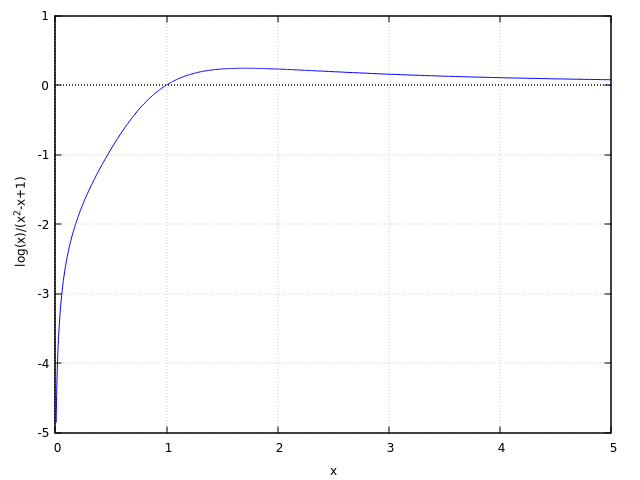
\includegraphics[scale=0.7]{images/interesting_integrals_06_3.png}
\end{figure}
